\section{\system Overview}
\begin{figure}[t]
	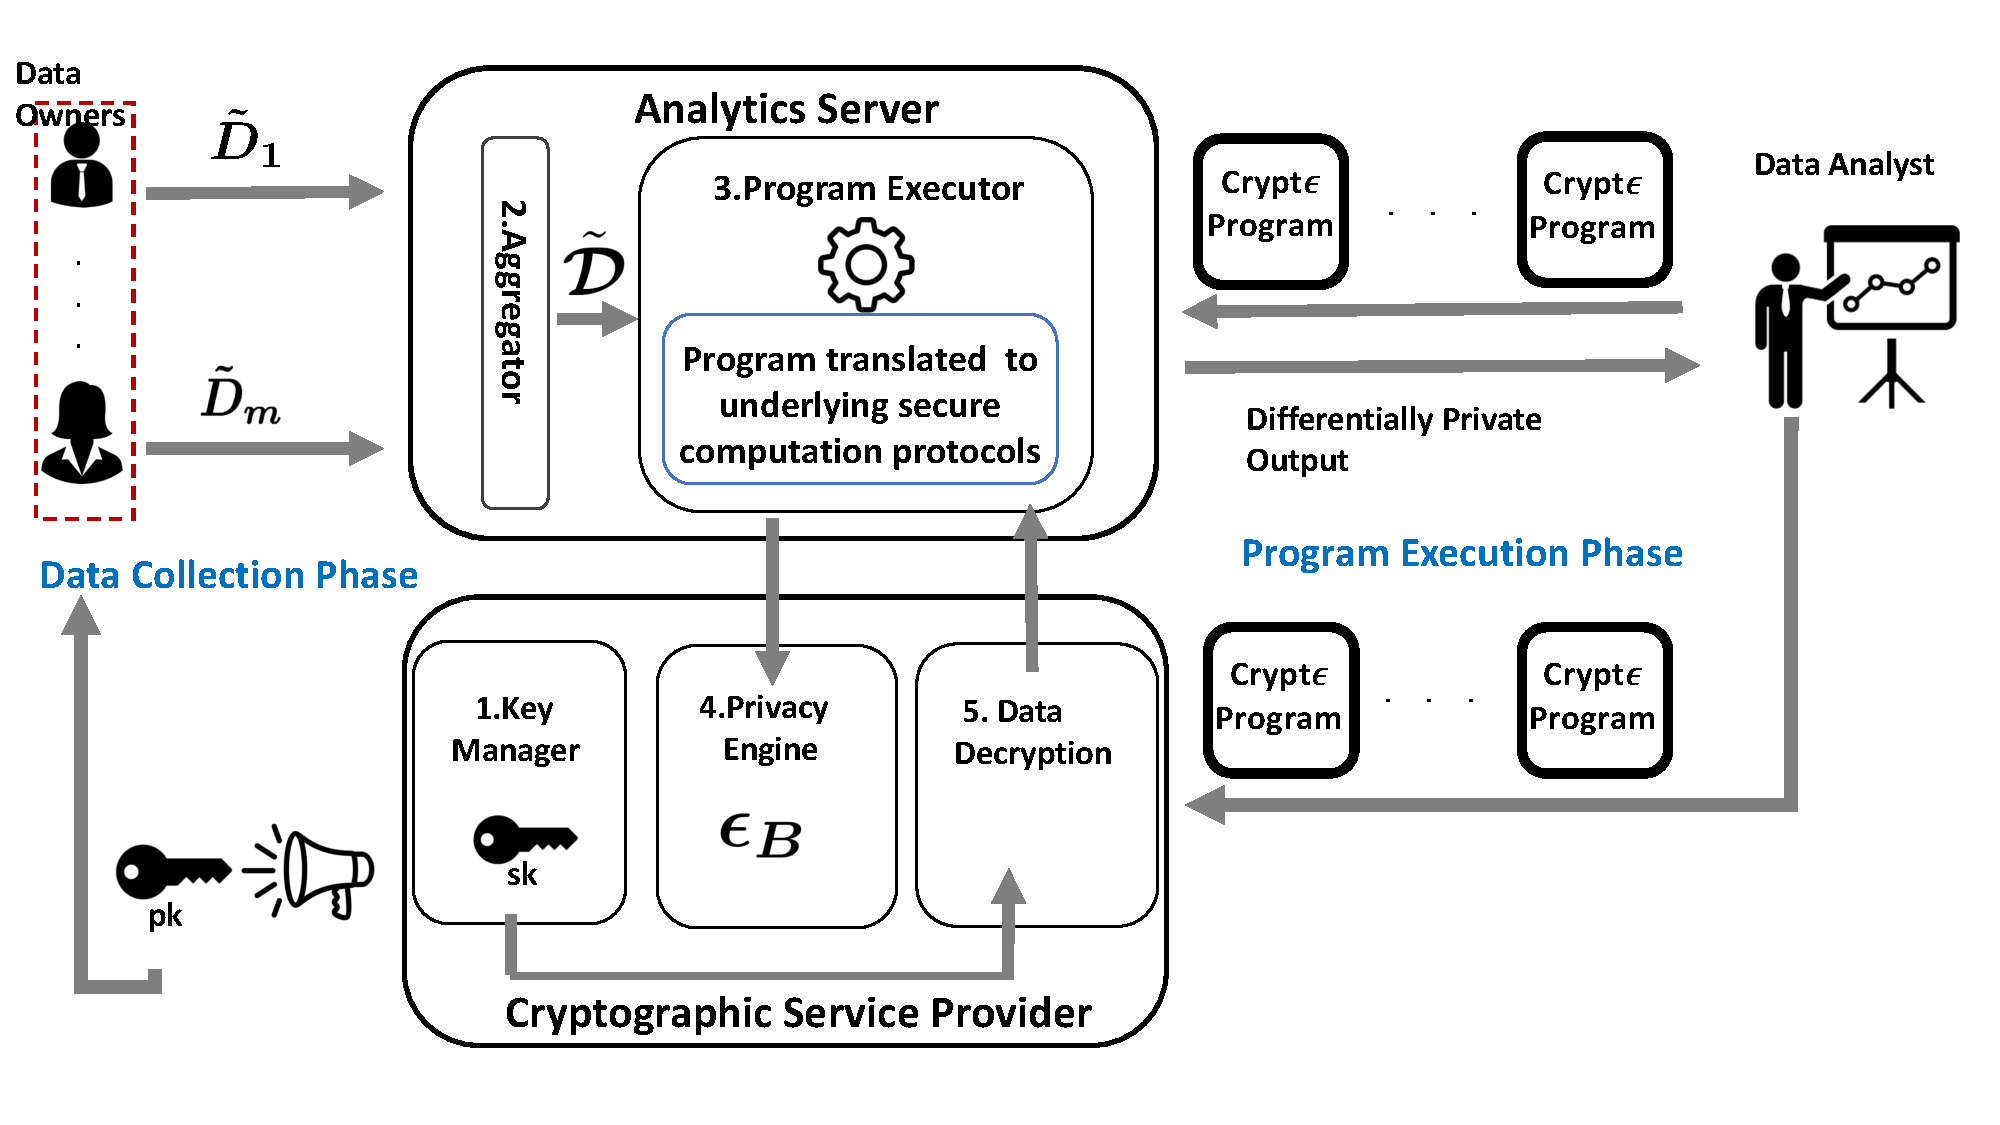
\includegraphics[width=0.7\columnwidth]{CryptE_Diag_New.pdf}\vspace{-5mm}
	\caption{\label{fig:system} Crypt$\epsilon$ System}% Setting: The  \textsf{AS} runs the Crypt$\epsilon$ programs. The \textsf{CSP} manages the cryptographic primitves. }
\end{figure}

\subsection{System Architecture}
Here we briefly review the system architecture of \system (illustrated by Fig \ref{fig:system}). %A set of \textit{data owners} ${\textsf{DO}_i, i\in [m]}$ have private data records ${D_i, i \in [m]}$. \system permits data analysts to author and execute programs $P$ that satisfy DP under the \cdp model without storing or computing on the private data records in the clear. 
At the very outset, the %\textit{Cryptographic Service Provider},
\CSP records the total privacy budget, $\epsilon^B$, (provided by the data owners) and generates the key pair $(pk,sk)$ (details in Section \ref{sec:background}) for the encryption scheme. The data owners, ${\textsf{DO}_i, i\in [m]}$, use the public key (pk) to encrypt their data records, ${D_i, i \in [m]}$, in the appropriate representation (per attribute one-hot-encoding, details in Section \ref{sec:overview}) and send the encrypted records, $\boldsymbol{\tilde{D_i}},i \in [m]$, to the \AS
which aggregates them into a single encrypted database $\encD$. Next, the \AS inputs logical programs from the data analysts and translates them to \system's underlying implementation specific secure computation protocols that work on $\encD$.  A \system program typically consists of a sequence of transformation operators followed by a measurement operator. A majority of the transformations are executed wholly at the \textsf{AS}.%The transformation operators are designed in such a way that the \AS can perform majority of the associated computation on its own. 
 However, every measurement operator requires an interaction with the \textsf{CSP} as it requires (a) decryption of the answer, and (b) a check that %the noise is scaled by the correct sensitivity (verified from the \system program) and that 
the total privacy budget, $\epsilon^B$, is not exceeded. In this way, the \AS and the \CSP can compute the output of a \system program with the data owners being offline during the  program execution. 
\vspace{-0.5cm}
\subsection{\system Design Principles}\label{sec:design}
\stitle{Minimal Trust Assumptions:} As mentioned above, the overarching goal of \system is to mimic the \cdp model but without a trusted server. A natural solution for dispensing with the trust assumption of the \cdp model is via cryptographic primitives \cite{Prochlo,mixnets,amplification,Shi,Shi2,kamara,Rastogi,DworkOurData,BeimelSFE+DP}. Hence, to accommodate the use of cryptographic primitives, we assume a computationally bounded adversary in \system. However, a generic $m+1$ party SMPC would be computationally unwieldy. This necessitates a third party entity that can capture the requisite secure computation functionality in (at least) a 2-party protocol instead. %Moreover, since the data owners are no longer in the loop to monitor every query answering, the aforementioned entity should also watchdog the overall privacy budget expenditure.
This role is essayed by the \CSP in \system. For this two-server model, we assume semi-honest behaviour and non-collusion. This is a very common assumption for privacy preserving computations in the two-server model \cite{Boneh1,Boneh2,Ridge2,Matrix2,secureML,LReg,Ver} and can be imposed in practice via legal bindings.

\stitle{Programming Framework:}
Conceptually, the aforementioned goal of achieving the \textit{best of both worlds} can be obtained by implementing the required DP program using off-the-self secure multi-party computation (SMPC) tools like \cite{EMP,MPCtools,ScaleMAMBA,ABY}. %This notion is similar in spirit with the works in \cite{DworkOurData,BeimelSFE+DP}. 
However, when it comes to real world deployment, \system trumps such approaches due to the following reasons.
 
 \textit{Firstly}, without the support of a programming framework like that of \system, the implementation of every DP program (corresponding to different data queries) has to be ad-hoc and from scratch resulting in high turnaround time. Moreover, the problem is compounded in our setting as executing DP programs on untrusted servers comes with additional challenges like tracking the  \textit{sensitivity} of each DP operation, monitoring of the  total privacy budget expenditure across all programs et al. %For example, revisiting our above mentioned database schema, let us assume that the data analyst is additionally interested in learning the output of a second query "Count the number of age values having at least 100 records". Typically, both of these queries will require two separate garbled circuits. 
Thus, in a practical query answering set-up, this is feasible only if %to be able to answer multiple queries on-the-fly
the data analyst is well-versed in both DP and SMPC techniques. In contrast, \system's programming framework empowers the data analyst
with an expressive language; consequently, for any program (supported by \system's language) in \system, the only task for an analyst is to encode the DP program logic in terms of the \system operators.  \system abstracts out all the low-level implementation details like the choice of input data representation, translating queries to that representation, choice of SMPC operators, key management, privacy budget monitoring etc
from the analyst thereby reducing his/her burden of complex decision making. Thus every program in \system is automatically translated to protocols corresponding to the underlying implementation. %In principle, any function can be computed on encrypted data via secure computation, and thus \system can support any differentially private algorithm. However, we currently limit the expressibility of the programs supported in \system to those that operate on the sensitive data with efficiently implementable operators, and whose privacy can be easily tracked by the \textsf{CSP}. Nevertheless, as shown later in the paper, \system can already support a rich class of state-of-the-art DP programs.%In fact, owing to this separation of the logical and physical layers, \system's underlying implementation can be based on cryptographic operators of choice. As mentioned above, in this paper we present a prototype \system that uses LHE and garbled circuits.

\textit{Secondly}, computation of naive SMPC protocols can be prohibitively costly for practical usage. Thus, the SMPC protocols corresponding to the different DP programs, have to be individually fine-tuned for performance improvement. In \system, on the other hand, %any optimization to an operator will be inherited by all programs using it. Thus 
ensuring optimal performance for just the small set of \system operators translates into practical efficiency for all \system programs. 

\textit{Thirdly}, a DP program can be typically divided into segments that perform noisy measurements of private data followed by segments of post-processing operations that can be performed in the clear. Thus, in order to implement a given DP program using SMPC operators, the data analyst has to first segregate the operations on the basis of whether it falls inside or outside the trust boundary. Otherwise, one has to implement the entire DP program inside a single protocol which will degrade performance. For  example, in the paper \cite{AHP}, the authors present an $\epsilon$-DP algorithm for releasing a histogram that works as follows. First, a preliminary estimate of the histogram, $\hat{H}$, is computed using budget $\epsilon_1$. This is followed by post-processing steps of thresholding, sorting and clustering $\hat{H}$ based on which the final histogram, $\tilde{H}$, is computed with the remaining privacy budget $\epsilon-\epsilon_1$. Implementing this entire algorithm in a single SMPC protocol would be extremely computation heavy; an implementation in EMP toolkit \cite{EMP} takes 810s for a dataset of size $\approx 33,000$.  On the other hand,
in \system the access to the sensitive data is limited via two measurement operators thereby making the separation between the trust boundaries in a program explicit. For the above example program, \system operators allow the computation of the two histograms, $\hat{H}$ and $\tilde{H}$ in a secure (private) fashion while the intermediate steps can be processed in the clear. A \system program for this takes 238s ($3.4\times$ less time than the EMP implementation)

\textit{Fourthly}, the security (privacy) proofs for just stand-alone cryptographic and DP mechanisms can be notoriously tricky \cite{BellareCryptoError,DPSVTProof}. Combining the two thus exacerbates the technical complexity, making the design vulnerable to faulty proofs \cite{He:2017:CDP}. For example, given any arbitrary DP program written under the \cdp model, the distinction between intermediate results that can be released beyond the trust boundary and the ones which has to be kept private is often ambiguous. An instance of this is observed in the Noisy-Max algorithm, where the array of intermediate noisy counts cannot be released.  However, note that these intermediate noisy counts in fact correspond to valid query responses. Thus, an incautious analyst, in a bid to improve performance, might reuse a previously released noisy count query output for a subsequent execution of the Noisy-Max algorithm leading to privacy leakage. In contrast, \system is designed to reveal nothing other than the outputs of the DP programs to the untrusted servers; every \system program comes with an automatic proof of security (privacy). Referring back to the aforementioned example, in \system, the Noisy-Max algorithm is implemented as a secure measurement operator thereby preventing any accidental privacy leakage. 


\stitle{Data Owners are Offline:}
 Recall, \system's goal is to mimic the \cdp model with untrusted  servers. Hence, it is designed so that the data owners are offline after submitting their encrypted records to the \textsf{AS}. %This is beneficial as the \textsf{AS} does not need to maintain communication channels with the data owners over a long period of time. 
 If the data owners were online, the efficiency of some programs could be improved as some of the computation %from the \textsf{AS} and \textsf{CSP} 
 can be offloaded to the data owners.



\stitle{Low burden on CSP:} \system views the \textsf{AS} as an extension of the analyst, and that it has a vested interest in obtaining the result of the computation.   Thus in \system, we require the \textsf{AS} to  shoulder the major chunk of the workload for any \system program execution; interactions with the \textsf{CSP} should be minimal and only related to data decryption. Keeping this in  mind, we design the \textsf{AS} to perform most of the data transformations by itself (Table \ref{perf}). Specifically for every Crypt$\epsilon$ program, the \textsf{AS} processes the whole database and transforms it into concise representations (like an encrypted scalar or a short vector) which is then decrypted with the help of the \textsf{CSP}. An example setting in the real world can be when Google assumes the role of the \AS and Symantec can provide the services of the \CSP. It is interesting to note that we could have had an alternative implementation for Crypt$\epsilon$ where the private database is equally shared between the two servers and they engage in a secret share based SMPC protocol for computing the DP answers. However, this would require both the servers to do almost equal amount of work for every program. Such an arrangement would be justified only if both the servers are equally invested in learning the DP statistics and is ill-suited for Crypt$\epsilon$. A real world analogy for this can be when Google and Baidu decide to compute some statistics on their combined user bases. We speculate that the above scenario is much less likely than the other setting. Additionally, oblivious transfer (OT) is the major bottleneck for most SMPC implementations \cite{OT:bottleneck:1,OT:bottleneck:2,OT:bottleneck:3} and in a secret share based computation, each AND (equivalently multiplication) gate involves an OT step. Thus a secret share based implementation would be much more communication intensive resulting in a performance hit. 

\stitle{Separation of logical programming framework and underlying physical implementation:} The programming framework is independent from the underlying cryptographic operator specific implementation. This allows certain flexibility in the choice for lower level physical implementation. 
 For example, the prototype \system presented in this paper, uses per attribute one-hot-encoding as the input data representation. However, one can easily switch over to any other encoding scheme like multi-attribute one-hot-encoding, range based encoding etc. %Quite evidently, different encoding scheme will have different storage requirements. For instance, a k-attribute one-hot-encoding will be of size $d^k$ where $d$ is the domain size of each attribute. We choose one-hot-coding for our prototype \system implementation because it is a general representation that can be easily translated to other encoding schemes.  
 Similarly, although in this paper, we use $\epsilon$-DP (pure DP) for our privacy analysis, \system can be easily extended to accommodate other DP notions like $(\epsilon,\delta)$-DP, R\`enyi differential privacy (RDP) \cite{RDP} etc. For example, designing an operator for adding Gaussian noise would suffice to allow RDP analysis in \system. As discussed above, due to our design choice of having low burden on the \CSP, we implement \system using LHE and garbled circuits. However translation to an implementation based on other cryptographic operators is straighforward. For example, the optimized HE scheme in \cite{Blatt2019OptimizedHE} can be used in place of LHE. Similarly, garbled circuits can be replaced by the mixed protocol ABY framework \cite{Demmler2015ABYA}. Of course, as mentioned above, a two server secret share based implementation is also possible. 


